\pagebreak
\begin{center}
    \rule{\textwidth}{1pt} \\[0.5cm]
    {\Huge \bfseries ANNEXES} \\[0.4cm]
    \rule{\textwidth}{1pt}
\end{center}


\label{demo1}
\begin{align*}
    \int_{-\infty}^{+\infty} g(t) \delta(t-t_0) dt = g(t_0)
\end{align*}
\begin{proof}
    \vspace{0.2cm}
    
    Soit $g$ une fonction continue en $t_0 \in \mathbb{R}$, on a :
    \begin{align*}
        \int_{-\infty}^{+\infty} g(t) \delta(t - t_0) dt = \lim_{\alpha \to 0+} \int_{-\infty}^{+\infty} g(t) f_{\alpha}(t - t_0) dt
    \end{align*}
    Soit $\alpha > 0$,
    \begin{align*}
        \int_{-\infty}^{+\infty} g(t) f_{\alpha}(t - t_0) dt &= \int_{t_0 - \alpha}^{t_0 + \alpha} \frac{g(t)}{2\alpha} dt \\
        &= \frac{1}{2 \alpha} \int_{t_0 - \alpha}^{t_0 + \alpha} g(t) dt \\
        &= \frac{1}{2 \alpha} \left( \int_{t_0 - \alpha}^{t_0 + \alpha} g(t_0) dt + \int_{t_0 - \alpha}^{t_0 + \alpha} \left( g(t) - g(t_0) \right) dt \right) \\
        &= g(t_0) + \frac{1}{2 \alpha} \int_{t_0 - \alpha}^{t_0 + \alpha} \left( g(t) - g(t_0) \right) dt
    \end{align*}
    Or, 
    \begin{align*}
        \left| \frac{1}{2 \alpha} \int_{t_0 - \alpha}^{t_0 + \alpha} \left( g(t) - g(t_0) \right) dt \right| &\leq \frac{1}{2 \alpha} \int_{t_0 - \alpha}^{t_0 + \alpha} \left| g(t) - g(t_0) \right| dt \\
        &\leq \sup_{t \in \left[ t_0 - \alpha ; t_0 + \alpha \right]} \left| g(t) - g(t_0) \right| \to 0 \quad \text{par continuité de g en $t_0$}
    \end{align*}

    Ainsi, on a bien $\lim_{\alpha \to 0+} \int_{-\infty}^{+\infty} g(t) f_{\alpha}(t - t_0) dt = g(t_0)$.

\end{proof}

\pagebreak

\label{demo2}
$$TFDI(TFD(x_n)) = x_n$$
\begin{proof}
    Soit $(x_0,x_1,...,x_{N-1}) \in \mathbb{C}^N$. Soit $0 \leq n < N$.

    \begin{align*}
        TFDI(TFD(x_n))&=\dfrac{1}{N} \sum_{k=0}^{N-1} \left(\sum_{m=0}^{N-1} x_m e^{-i \frac{2\pi}{N} km}\right) e^{i \frac{2 \pi}{N}kn} \\
        &= \dfrac{1}{N} \sum_{m=0}^{N-1} x_m \left( \sum_{k=0}^{N-1} e^{-i \frac{2\pi}{N} k(m-n)} \right)
    \end{align*}
    Posons :
    $$S_N \coloneq \sum_{k=0}^{N-1}e^{-i \frac{2\pi}{N} k(m-n)}$$
    On remarque que $S_N$ est une somme partielle d'une suite géométrique de raison $q = e^{-i \frac{2\pi}{N} (m-n)}$.
    \begin{description}
        \item[Si $n=m$, ] $q = e^0 = 1 \implies S_N = \sum_{k=0}^{N-1} 1 = N$  
        \item[Si $n\neq m$, ] $S_N=\frac{1-q^N}{1-q}$ or, $q^N = e^{-i2\pi(m-n)} = 1$ car $m-n\in \mathbb{Z}$ donc $S_N = 0$ 
    \end{description}
    $$\implies TFDI(TFD(x_n)) =\dfrac{1}{N}\sum_{m=0}^{N-1}x_m \cdot N \delta_{nm} = \dfrac{1}{N}x_n\cdot N = x_n$$
\end{proof}

\pagebreak

\label{demo3}
Les $ e_k(n) = \alpha_k \cos\left(\frac{\pi}{N}\left(n+\frac{1}{2}\right)k\right),\quad k=0,\dots,N-1 $ forment une base orthonormale pour le produit scalaire usuel sur $\mathbb{R}^N$.
\begin{proof}
    On considère le produit scalaire usuel sur $\mathbb{R}^N$ :
    $ \langle x,y\rangle = \sum_{n=0}^{N-1} x_ny_n $
    On calcule :
    $$
        \langle e_k,e_l\rangle = \alpha_k \alpha_l \sum_{n=0}^{N-1} \cos\left(\frac{\pi}{N}\left(n+\frac{1}{2}\right)k\right) \cos\left(\frac{\pi}{N}\left(n+\frac{1}{2}\right)l\right)
    $$

        On remarque alors que $\sum_{n=0}^{N-1} \cos\left(\theta\left(n + \frac{1}{2}\right)\right) = \frac{\sin(N\theta/2)}{2\sin(\theta)}$, d'où :
    \begin{align*}
        \langle e_k,e_l\rangle
        &= \frac{\alpha_k \alpha_l}{2} \left( \frac{\sin(N(\theta_k - \theta_l))}{2\sin((\theta_k - \theta_l)/2)} + \frac{\sin(N(\theta_k + \theta_l))}{2\sin((\theta_k + \theta_l)/2)} \right) \\
        &= \frac{\alpha_k \alpha_l}{4} \left( \frac{\sin(\pi(k-l))}{\sin(\pi(k-l)/2N)} + \frac{\sin(\pi(k+l))}{\sin(\pi(k+l)/2N)} \right)
    \end{align*}
\begin{itemize}
    \item Si $k \neq l$, alors $\langle e_k,e_l\rangle = \sin(\pi(k-l)) = \sin(\pi(k+l)) = 0$
    \item Si $k=l \neq 0$, le premier terme vaut $2N$ et le second est nul :
    $\langle e_k,e_k\rangle = \frac{\alpha_k^2}{4} 2N = \frac{1}{2N}2N= 1$
    \item Si $k=l=0$, les deux termes valent $2N$ par continuité en 0 :
    $\langle e_0,e_0\rangle = \frac{\alpha_0^2}{4} (2N + 2N) = 1$
\end{itemize}

    Ainsi, la famille $(e_k)$ forme une base orthonormale de $\mathbb{R}^N$.
\end{proof}

\pagebreak

\label{demo4}
$$IDCT(DCT(x_n)) = x_n$$
\begin{proof}
    On a, par définition,
    \begin{align*}
        X_k = \alpha_k\sum_{m=0}^{N-1}x_m\cos \left[\frac{\pi}{N}\left(m+\frac{1}{2}\right)k\right] \\
        x_n = \sum_{k=0}^{N-1}\alpha_k X_k\cos \left[\frac{\pi}{N}\left(n+\frac{1}{2}\right)k\right]\\
    \end{align*}
    On développe, 
    \begin{align*}
        IDCT(DCT(x_n))&=\sum_{k=0}^{N-1}\alpha_k \left(\alpha_k\sum_{m=0}^{N-1}x_m\cos \left[\frac{\pi}{N}\left(m+\frac{1}{2}\right)k\right]\right)\cos \left[\frac{\pi}{N}\left(n+\frac{1}{2}\right)k\right]\\
        &=\sum_{k=0}^{N-1}\left(\alpha_k^2\sum_{m=0}^{N-1}x_m\cos \left[\frac{\pi}{N}\left(m+\frac{1}{2}\right)k\right]\right)\cos \left[\frac{\pi}{N}\left(n+\frac{1}{2}\right)k\right]\\
        &=\sum_{m=0}^{N-1}x_m\left(\sum_{k=0}^{N-1}\alpha_k^2\cos \left[\frac{\pi}{N}\left(m+\frac{1}{2}\right)k\right]\cos \left[\frac{\pi}{N}\left(n+\frac{1}{2}\right)k\right]\right)\\
        &=\sum_{m=0}^{N-1}x_m\left(\sum_{k=0}^{N-1}\left(\alpha_k\cos \left[\frac{\pi}{N}\left(m+\frac{1}{2}\right)k\right]\right)\left(\alpha_k\cos \left[\frac{\pi}{N}\left(n+\frac{1}{2}\right)k\right]\right)\right) \\
    \end{align*}
    Posons $e_i(k) =\alpha_k\cos\left[\frac{\pi}{N}\left(i+\frac{1}{2}\right)k\right], e_i=(e_i(0),e_i(1), \dots ,e_i(N-1)) \in \mathbb{R}^N$, alors,
    \begin{align*}    
        IDCT(DCT(x_n)) &=\sum_{m=0}^{N-1}x_m\left(\sum_{k=0}^{N-1}e_m(k)e_n(k)\right) \\
        &=\sum_{m=0}^{N-1}x_m\langle e_m,e_n\rangle =\sum_{m=0}^{N-1}x_m\delta_{m,n} = x_n
    \end{align*}
\end{proof}

\pagebreak

\label{demo5}
Les basses fréquences sont situées dans les coins du spectre. 

\begin{proof}
    En effet, les fréquences discrètes étant périodiques, on peut les représenter sur un tore discret. Ainsi, les coins ne sont pas proches sur le spectre visuellement mais sont mathématiquement adjacents grâce à leur périodicité modulo $N$ et $M$. On peut alors définir une distance sur ce tore en tirant parti de la symétrie modulo $N$ : $d_N(x, y) = \min(|x - y| \pmod N, N - (|x - y| \pmod N))$ (pareil dans l'autre direction avec $M$). Ainsi, on peut mesurer la distance d'un point par rapport à l'origine en faisant $d_N(k,0)=\min(k,N-k)$.
\begin{figure}[H]
    \centering
    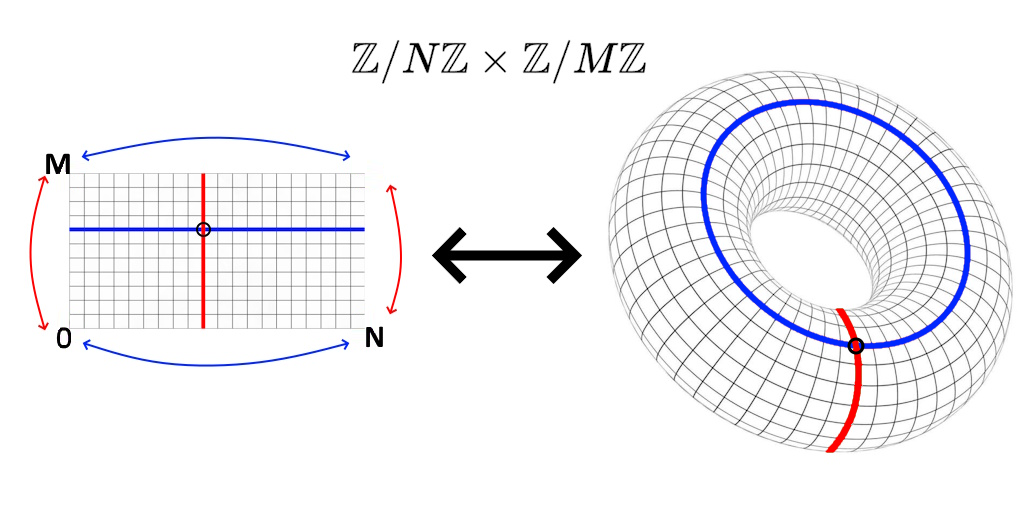
\includegraphics[width=0.75\textwidth]{images/Tore.png}
    \caption{Représentation visuelle en tore}
\end{figure}
Soient $k \in \{0, \dots, M-1\}$ et $l \in \{0, \dots, N-1\}$ \\
Posons $\varphi_{k,l}: \mathbb{Z}/N\mathbb{Z} \times  \mathbb{Z}/M\mathbb{Z} \to \mathbb{C}$ telle que $\varphi_{k,l}(n,m)=\exp(-2i\pi (\frac{kn}{N} + \frac{lm}{M}))$
Nous pouvons alors étudier le taux d'accroissement entre deux fréquences discrètes.
$$\frac{\varphi_{k,l}(n+1,m)}{\varphi_{k,l}(n,m)} = \frac{\exp(-2i\pi (\frac{k(n+1)}{N} + \frac{lm}{M}))}{\exp(-2i\pi (\frac{kn}{N} + \frac{lm}{M}))} = e^{\frac{-2i\pi k}{N}}$$
Ainsi, \\
$d_N(k,0) \ll N \implies |\frac{2\pi k}{N}|\ll 1 \implies e^{\frac{-2i \pi k}{N}} \approx 1 \implies \varphi_{k,l}(n+1,m) \approx \varphi_{k,l}(n,m)$ \\
$k \approx \frac{N}{2} \implies e^{\frac{-2i \pi k}{N}} \approx -1 \implies \varphi_{k,l}(n+1,m) \approx -\varphi_{k,l}(n,m)$
Plus la distance $d_N(k,0)$ est faible, moins la fonction présente d'oscillations, ce qui traduit la présence de basses fréquences. À l'inverse, plus $k$ est proche de $\frac{N}{2}$, plus la fonction oscille rapidement, ce qui correspond à des hautes fréquences.Par un raisonnement analogue sur l'accroissement dans la seconde direction (selon l'indice $l$ et la dimension $M$), on montre que les variations spatiales suivent la même logique.En conclusion, les fréquences les plus faibles (les composantes continues et lentes du signal) se concentrent autour de l'origine et, par périodicité modulo $N$ et $M$, se retrouvent également dans les quatre coins du spectre discret.
\end{proof}

\pagebreak


\label{demo6}
\begin{proof}
    Soit $f$ une image de taille $M \times N$, représentée par une matrice de pixels où $f(n, m) \in \mathbb{C}$ est l'intensité du pixel à la position $(n, m)$. \\
    On étudie le spectre de l'image (appartenant à $\mathbb{C}^{M\times N}$) par une transformée de Fourier discrète (FFT). \\
    On considère le produit scalaire standard sur cet espace : 
    $$ \langle f,g \rangle = \sum_{n=0}^{M-1}\sum_{m=0}^{N-1}f(n,m)\overline{g(n,m)}$$
    On définit une distance sur cet espace en tirant parti de la symétrie modulo $M$ (respectivement $N$) : $d_M(x, y) = \min(|x - y| \pmod M, M - (|x - y| \pmod M))$. Ainsi, on mesure la distance d'un point par rapport à l'origine en faisant $d_M(k,0)=\min(k,M-k)$. \\
    Soient $k \in \{0, \dots, M-1\}$ et $l \in \{0, \dots, N-1\}$. Les fonctions $\varphi_{k,l}: \mathbb{Z}/M\mathbb{Z} \times \mathbb{Z}/N\mathbb{Z} \to \mathbb{C}$ telles que $\varphi_{k,l}(n,m)=\exp\left(-2i\pi \left(\frac{kn}{M} + \frac{lm}{N}\right)\right)$ forment une base orthogonale de $\mathbb{C}^{M\times N}$.
    
    Posons $R \in [0,1]$ le ratio de conservation des fréquences pour l'image.
    Comme $\mathbb{C}^{M\times N}$ est un espace vectoriel de dimension finie, on peut écrire la décomposition unique : 
    $$f = f_R + h \quad \text{avec} \quad f_R \in V_R, \, h \in V_R^{\perp}$$ 
    où $V_R = \text{Vect}\left(\left\{\varphi_{k,l} \mid d_M(k,0) \leq R \cdot M \text{ et } d_N(l,0) \leq R \cdot N\right\}\right)$.
    Soit $g \in V_R$ \\
    $$f-g=(f_R+h)-g=(f_R-g)+h$$ or $f_R-g \in V_R$ et $h \in V_R^{\perp}$ donc $\langle f_R-g, h \rangle = 0$ \\
    D'après le théorème de Pythagore : 
    \begin{align*}
        \lVert f-g \rVert^2 &= \lVert f_R-g \rVert^2 + \lVert h \rVert^2 \\
                            &\implies \lVert f-g \rVert^2 \geq \lVert h \rVert^2 \\
                            &\implies (\lVert f-g \rVert^2 = \lVert h \rVert^2 \iff g = f_R) \\
                            &\implies \lVert f-f_R \rVert^2 = \min_{g \in V_R} \lVert f-g \rVert^2
    \end{align*}
    Ainsi, la fonction minimisant l'erreur $\lVert f-f_R \rVert^2$ est la fonction g qui est donc le projeté orthogonal sur le sous-espace vectoriel $V_R$ formé par les $\varphi_{k,l}$ ayant leurs $k$ et $l$ proches de l'origine. C'est donc l'hyperplan formé par les fréquences les plus basses. Il faut ainsi conserver les fréquences faibles pour compresser une image à l'aide d'une FFT.
    
\end{proof}